\documentclass[11pt]{article}
\usepackage{acl2012}
\usepackage{times}
\usepackage{latexsym}
\usepackage{amsmath}
\usepackage{multirow}
\usepackage{url}
\usepackage{graphicx}
\usepackage[usenames,dvipsnames]{pstricks}
\usepackage{epsfig}
\DeclareMathOperator*{\argmax}{arg\,max}
\setlength\titlebox{6.5cm}    % Expanding the titlebox

\title{Learning Syntactic Categories Using Paradigmatic Representations}

\author{First Author \\
  Affiliation / Address line 1 \\
  Affiliation / Address line 2 \\
  Affiliation / Address line 3 \\
  {\tt email@domain} \\\And
  Second Author \\
  Affiliation / Address line 1 \\
  Affiliation / Address line 2 \\
  Affiliation / Address line 3 \\
  {\tt email@domain} \\\And
  Third Author \\
  Affiliation / Address line 1 \\
  Affiliation / Address line 2 \\
  Affiliation / Address line 3 \\
  {\tt email@domain} \\}

\date{}

\begin{document}
\maketitle
\begin{abstract}
We introduce a paradigmatic representation of word context and
demonstrate its utility in learning syntactic categories.  Unlike the
typical syntagmatic representations of word context which consist of
properties of neighboring words, our paradigmatic representation
consists of substitute vectors: possible substitutes of the target
word and their probabilities.  When word contexts are clustered based
on their substitute vectors they reveal a grouping that largely match
the traditional part of speech boundaries with a many-to-one accuracy
of \collapseResult\% on a 45-tag 24K word test corpus.
\end{abstract}

\section{Introduction}
\label{sec:intro}

Grammar rules apply not to individual words (e.g. dog, eat) but to
syntactic categories of words (e.g. noun, verb).  Thus constructing
syntactic categories (also known as lexical or part-of-speech
categories) is one of the fundamental problems in language
acquisition.

Linguists identify syntactic categories based on semantic, syntactic,
and morphological properties of words.  There is also evidence that
children use prosodic and phonological features to bootstrap syntactic
category acquisition \cite{ambridge2011child}.  However there is as
yet no satisfactory computational model that can match human
performance.  Thus identifying the best set of features and best
learning algorithms for syntactic category acquisition is still an
open problem.

Computational models of syntactic category acquisition in the
literature mainly rely on distributional analysis: Items that share
the same distribution (i.e. that occur in the same context) are
grouped into the same category.  The definition of ``the same
context'' vary across studies.  Algorithms based on the Hidden Markov
Model use class based n-grams to specify context
\cite{Brown:1992:CNG:176313.176316}, others use a frame of neighboring
words around the target word \cite{Schutze:1995:DPT:976973.976994}.
Our main contribution in this study is to introduce paradigmatic
features, i.e. features based on potential substitutes of the target
word, to represent word context.

Relationships between linguistic units can be classified into two
types: syntagmatic (concerning positioning), and paradigmatic
(concerning substitution).  Syntagmatic relations determine which
units can combine to create larger groups and paradigmatic relations
determine which units can be substituted for one another.
Figure~\ref{fig:paradigmatic} illustrates the paradigmatic vs
syntagmatic axes for words in a simple sentence and their possible
substitutes.

\begin{figure}[h] \centering
% Generated with LaTeXDraw 2.0.8
% Tue Jan 10 15:57:06 EET 2012
% \usepackage[usenames,dvipsnames]{pstricks}
% \usepackage{epsfig}
% \usepackage{pst-grad} % For gradients
% \usepackage{pst-plot} % For axes
\scalebox{1} % Change this value to rescale the drawing.
{
\begin{pspicture}(0,-1.6728125)(4.73474,1.6528125)
\usefont{T1}{ptm}{m}{n}
\rput(0.39520833,-0.6571875){\psframebox[linewidth=0.04]{the}}
\usefont{T1}{ptm}{m}{n}
\rput(1.8816146,-0.6571875){\psframebox[linewidth=0.04]{man}}
\usefont{T1}{ptm}{m}{n}
\rput(1.9886458,0.3428125){\psframebox[linewidth=0.04,linestyle=dashed,dash=0.16cm 0.16cm]{girl}}
\usefont{T1}{ptm}{m}{n}
\rput(3.3298957,-0.6571875){\psframebox[linewidth=0.04]{cried}}
\usefont{T1}{ptm}{m}{n}
\rput(3.2798958,0.3428125){\psframebox[linewidth=0.04,linestyle=dashed,dash=0.16cm 0.16cm]{died}}
\usefont{T1}{ptm}{m}{n}
\rput(3.3158333,1.3428125){\psframebox[linewidth=0.04,linestyle=dashed,dash=0.16cm 0.16cm]{sang}}
\usefont{T1}{pcr}{m}{n}
\rput(2.020677,-1.4671875){\footnotesize syntagmatic axis}
\usefont{T1}{pcr}{m}{n}
\rput{-90.0}(4.4150524,4.661927){\rput(4.507552,0.1328125){\footnotesize paradigmatic axis}}
\psline[linewidth=0.04cm,arrowsize=0.05291667cm 2.0,arrowlength=1.4,arrowinset=0.4]{<->}(0.13364583,-1.1671875)(3.9336457,-1.1671875)
\psline[linewidth=0.04cm,arrowsize=0.05291667cm 2.0,arrowlength=1.4,arrowinset=0.4]{<->}(4.133646,1.6328125)(4.133646,-1.1671875)
\psline[linewidth=0.04cm](0.81364584,-0.6671875)(1.4136459,-0.6671875)
\psline[linewidth=0.04cm](2.3936458,-0.6671875)(2.8136458,-0.6671875)
\psline[linewidth=0.04cm](1.9136459,0.0528125)(1.9136459,-0.4271875)
\psline[linewidth=0.04cm](3.3136458,0.0928125)(3.3136458,-0.3671875)
\psline[linewidth=0.04cm](3.3136458,1.0128125)(3.3136458,0.6328125)
\end{pspicture} 
}

\caption{Syntagmatic vs. paradigmatic axes for words in a simple
  sentence \cite{chandler2007semiotics}.}
\label{fig:paradigmatic}
\end{figure}

Both syntagmatic and paradigmatic relations of a word can be used to
represent its context.  In the syntagmatic case the context is
represented by a selection of neighboring words, in the paradigmatic
case it is represented by a set of possible substitutes.  In previous
studies of syntactic category learning the context representation has
been primarily syntagmatic, either implicit in the class based n-grams
of the standard Hidden Markov Model, or explicit in the construction
and clustering of left and right neighbors.

In this study we explore a paradigmatic representation of the context
of a word in syntactic category acquisition.  Specifically, the
context of a word is represented by a list of its possible substitutes
and their probabilities, which we call the {\em substitute vector}.
Note that the substitute vector is a function of the context only, not
the target word.  Thus in effect we are clustering contexts, not
words.  When word contexts are clustered based on their substitute
vectors they reveal a grouping that largely match the traditional part
of speech boundaries (\collapseResult\% many-to-one score using a
45-tag 24K word test corpus).
% standard HMM-EM gives 42\% on the same data.

Section~\ref{sec:related} gives a detailed review of related work.
The construction of the substitute vectors is described in
Section~\ref{sec:lm}.  To find out how to best make use of this new
paradigmatic representation, we explore different distance metrics
(Section~\ref{sec:dist}), dimensionality reduction methods
(Section~\ref{sec:dimreduce}), and clustering algorithms
(Section~\ref{sec:clustering}) for substitute vectors.  We note that
close to 95\% of the word occurrences in human labeled data are tagged
with their most frequent part of speech
\cite{Lee:2010:STU:1870658.1870741}, making one-tag-per-word a fairly
good first approximation.  Even ambicategory words generally have
fairly skewed part of speech distributions.
Section~\ref{sec:sparsity} looks at ways to increase the sparsity of
our solutions and demonstrates significant improvements using the
one-tag-per-word assumption and similarity metrics that introduce
sparsity.  Section~\ref{sec:discussion} discusses the results and
Section~\ref{sec:contrib} summarizes our contributions.


\section{Related Work}
\label{sec:related}

There are several good reviews of algorithms for unsupervised
part-of-speech induction
\cite{Christodoulopoulos:2010:TDU:1870658.1870714,Gao:2008:CBE:1613715.1613761}
and models of syntactic category acquisition \cite{ambridge2011child}.
In this review we focus on (i) the information captured by the inputs,
and (ii) the constraints applied to the outputs of the algorithms.

This work is to be distinguished from supervised part-of-speech
disambiguation systems, which use labeled training data
\cite{Church:1988:SPP:974235.974260}, unsupervised disambiguation
systems, which use a dictionary of possible tags for each word
\cite{Merialdo:1994:TET:972525.972526}, or prototype driven systems
which use a small set of prototypes for each class
\cite{Haghighi:2006:PLS:1220835.1220876}.  The problem of induction is
important for studying under-resourced languages that lack labeled
corpora and high quality dictionaries.  It is also essential in
modeling child language acquisition because every child manages to
induce syntactic categories without access to labeled sentences,
labeled prototypes, or dictionary constraints.

\paragraph{Clustering vs. HMMs:}
Models of unsupervised induction of part-of-speech categories fall
into two broad groups.  The first group uses algorithms that cluster
word types based on their context statistics
\cite{Schutze:1995:DPT:976973.976994}.  Work in modeling child
syntactic category acquisition has generally followed this clustering
approach \cite{redington1998distributional,mintz2003frequent}.  The
second group consists of probabilistic models based on the Hidden
Markov Model (HMM) framework \cite{Brown:1992:CNG:176313.176316}.

\paragraph{Clustering and data sparsity:}
Clustering based methods represent context using neighboring words,
typically a single word on the left and a single word on the right
called a ``frame'' (e.g., {\em {\bf the} dog {\bf is}; {\bf the} cat
  {\bf is}}).  They cluster word types rather than word tokens based
on the frames they occupy thus employing one-tag-per-word assumption
from the beginning (with the exception of some methods in
\cite{Schutze:1995:DPT:976973.976994}).  They may suffer from data
sparsity caused by infrequent words and infrequent contexts.  The
solutions suggested either restrict the set of words and set of
contexts to be clustered to the most frequently observed or use
dimensionality reduction.  \cite{redington1998distributional} defines
context similarity based on the number of common frames bypassing the
data sparsity problem but achieves mediocre results.
\cite{mintz2003frequent} only uses the most frequent 45 frames and
\cite{biemann2006unsupervised} clusters the most frequent 10,000 words
using contexts formed from the most frequent 150-200 words.
\cite{Schutze:1995:DPT:976973.976994,lamar-EtAl:2010:Short} employ SVD
to enhance similarity between less frequently observed words and
contexts.  \cite{Lamar:2010:LCU:1870658.1870736} represents each
context by the currently assigned left and right tag (which eliminates
data sparsity) and clusters word types using a soft k-means style
iterative algorithm.  They report the best clustering result to date
of 70.8\% many-to-one accuracy on a 45-tag 1M word corpus.

% all except schutze cluster word types

\paragraph{HMMs and distribution sparsity:}
The prototypical bitag HMM model maximizes the likelihood of the
corpus $w_1 \ldots w_n$ expressed as $P(w_1|c_1)\prod_{i=2}^n
P(w_i|c_i) P(c_i|c_{i-1})$ where $w_i$ are the word tokens and $c_i$
are their (hidden) tags.  One problem with such a model is its
tendency to distribute probabilities equally and the resulting
inability to model highly skewed word-tag distributions observed in
hand-labeled data \cite{johnson:2007:EMNLP-CoNLL2007}.  To favor
sparse word-tag distributions one can enforce a strict
one-tag-per-word solution
\cite{Brown:1992:CNG:176313.176316,Clark:2003:CDM:1067807.1067817},
use sparse priors in a Bayesian setting
\cite{goldwater-griffiths:2007:ACLMain,johnson:2007:EMNLP-CoNLL2007},
or use posterior regularization
\cite{Ganchev:2010:PRS:1859890.1859918}.  Each of these techniques
provide significant improvements over the standard HMM model: for
example \cite{Gao:2008:CBE:1613715.1613761} shows that sparse priors
can gain from 4\% (62\% to 66\% with a 1M word corpus) to 30\% (28\%
to 58\% with a 24K word corpus) in cross-validated many-to-one
accuracy.  However \cite{Christodoulopoulos:2010:TDU:1870658.1870714}
shows that the older one-tag-per-word models such as
\cite{Brown:1992:CNG:176313.176316} outperform the more sophisticated
sparse prior and posterior regularization methods both in speed and
accuracy (the Brown model gets 68\% many-to-one accuracy with a 1M
word corpus).  Given that close to 95\% of the word occurrences in
human labeled data are tagged with their most frequent part of speech
\cite{Lee:2010:STU:1870658.1870741}, this is probably not surprising;
one-tag-per-word is a fairly good first approximation for induction.

\paragraph{Poverty of features:}
Another problem with the plain HMM model is the poverty of its input
features.  Of the syntactic, semantic, and morphological information
linguists claim underlie syntactic categories, bitag HMMs only
represent limited syntactic information in their class based n-grams.
\cite{Clark:2003:CDM:1067807.1067817,bergkirkpatrick-klein:2010:ACL,blunsom-cohn:2011:ACL-HLT2011}
incorporate similar orthographic features and report improvements of
3, 7, and 10\% respectively over the baseline Brown model.
\cite{Christodoulopoulos:2010:TDU:1870658.1870714} use prototype based
features as described in \cite{Haghighi:2006:PLS:1220835.1220876} with
automatically induced prototypes and report an 8\% improvement over
the baseline Brown model.  Semantic information is incorporated to
some extent by some clustering based models and our paradigmatic
model.  To our knowledge, nobody has yet tried to incorporate
phonological or prosodic features in a computational model for
syntactic category acquisition.

\paragraph{Evaluation:}
It is natural to question the merit of evaluating unsupervised results
by comparing them to gold standard tags.  For example
\cite{freudenthal2005resolution} argue that a verb category (such as
{\sc vb} in Penn Treebank) that contains verbs that can and cannot be
used in certain constructions (e.g. the imperative) and verbs that can
be used as both auxiliaries and main verbs (e.g., {\em do, have}) does
not in fact constitute a set of items that could be substituted for
one another in particular sentences.  Such a category fails the
standard linguistic definition of a syntactic category and children do
not seem to make errors of substituting such words in utterances
(e.g. {\em''What do you want?''} vs. {\em *''What put you want?''}).
They suggest evaluating models by incorporating a production component
that allows the model's output to be compared to speech produced by
children exposed to the same input.  \cite{frank2009evaluating},
motivated by the lack of gold standards for many novel languages,
suggest comparing a system's clusters to a set of clusters created
from {\em substitutable frames}.  They create frames using two words
appearing in the corpus with exactly one word between and calculate
precision, recall, and F-score of the system's clustering.
Statistical parsers or factored machine learning systems could also be
sources of extrinsic evaluation for induced syntactic categories.  We
hope such extrinsic evaluation will be more widespread in the future
but nevertheless use the 45-tag Penn Treebank gold standard to
evaluate the current work.

\paragraph{Our work:}
Our work is more closely related to clustering based methods with two
important differences: (i) we represent word contexts not by an ad-hoc
selection of syntagmatic features based on a single word neighborhood
but by substitute vectors defined by a statistical language model
representing paradigmatic features of a larger window, (ii) we cluster
word tokens (or rather their contexts) instead of word types, which
means not being constrained by the one-tag-per-word assumption from
the beginning.  The features in our model incorporate semantic as well
as syntactic information from the context as illustrated by the
examples in Section~\ref{sec:lm}.  Our best results on the 45-tag 24K
corpus given in Section~\ref{sec:sparsity} (\collapseResult\% many-to-one)
compare favorably with best previously reported results on the same
corpus (58.2\% in \cite{Gao:2008:CBE:1613715.1613761}).  This
significant improvement is due to the additional information obtained
from the statistical language model which also comes at a great
computational cost.  Developing faster algorithms to find high
probability substitutes is in our current research agenda.

\section{Substitute Vectors}
\label{sec:lm}

In this study, we predict the part of speech of a word in a given
context based on its substitute vector.  The dimensions of the
substitute vector represent words in the vocabulary, and the entries
in the substitute vector represent the probability of those words
being used in the given context.  Note that the substitute vector is a
function of the context only and is indifferent to the target word.
This section details the choice of the data set, the vocabulary and
the estimation of substitute vector probabilities.

% what is the test data
The Wall Street Journal Section of the Penn Treebank \cite{treebank3}
was used as the test corpus (1,173,766 tokens, 49,206 types).
% what is the tag set
The treebank uses 45 part-of-speech tags which is the set we used as
the gold standard for comparison in our experiments.
% what is the LM training data
%Train => 5181717 126019973 690121813
To compute substitute probabilities we trained a language model using
approximately 126 million tokens of Wall Street Journal data
(1987-1994) extracted from CSR-III Text \cite{csr3text} (we excluded
the test corpus).
% how is the language model trained
We used SRILM \cite{Stolcke2002} to build a 4-gram language model with
Kneser-Ney discounting.
% what is the vocabulary
Words that were observed less than 20 times in the LM training data
were replaced by \textsc{unk} tags, which gave us a vocabulary size of
78,498.
% perplexity
The perplexity of the 4-gram language model on the test corpus is 96.

% how are the substitutes computed
It is best to use both left and right context when estimating the
probabilities for potential lexical substitutes.  For example, in
\emph{``He lived in San Francisco suburbs.''}, the token \emph{San}
would be difficult to guess from the left context but it is almost
certain looking at the right context.  We define $c_w$ as the $2n-1$
word window centered around the target word position: $w_{-n+1} \ldots
w_0 \ldots w_{n-1}$ ($n=4$ is the LM order).  The probability of a
substitute word $w$ in a given context $c_w$ can be estimated as:
\begin{eqnarray}
  \label{eq:lm1}P(w_0 = w | c_w) & \propto & P(w_{-n+1}\ldots w_0\ldots w_{n-1})\\
  \label{eq:lm2}& = & P(w_{-n+1})P(w_{-n+2}|w_{-n+1})\nonumber\\
  &&\ldots P(w_{n-1}|w_{-n+1}^{n-2})\\
  \label{eq:lm3}& \approx & P(w_0| w_{-n+1}^{-1})P(w_{1}|w_{-n+2}^0)\nonumber\\
  &&\ldots P(w_{n-1}|w_0^{n-2})
\end{eqnarray}
where $w_i^j$ represents the sequence of words $w_i w_{i+1} \ldots
w_{j}$.  In Equation \ref{eq:lm1}, $P(w|c_w)$ is proportional to
$P(w_{-n+1}\ldots w_0 \ldots w_{n+1})$ because the words of the
context are fixed.  Terms without $w_0$ are identical for each
substitute in Equation \ref{eq:lm2} therefore they have been dropped
in Equation \ref{eq:lm3}.  Finally, because of the Markov property of
n-gram language model, only the closest $n-1$ words are used in the
experiments.

For computational efficiency only the top 100 substitutes and their
unnormalized probabilities were computed for each of the 1,173,766
positions in the test set using the {\sc fastsubs} algorithm described
in \cite{selfcitation}\footnote{{\sc fastsubs} accomplishes this task
  in about 5 hours, a naive algorithm that looks at the whole
  vocabulary would take more than 6 days on a typical 2012
  workstation.}.  The probability vectors for each position were
normalized to add up to 1.0 giving us the final substitute vectors
used in the rest of this study.

% example substitute vectors (both syntactic and semantic)
The high probability substitutes reflect both semantic and syntactic
features of the context as seen in the examples given in
Table~\ref{tab:subs}.  Top substitutes for the word ``the'' consist of
words that can act as determiners.  Top substitutes for ``board'' are
not only nouns, but specifically nouns compatible with the semantic
context.

\begin{table}[h]\centering
\begin{tabular}{|l|ll|} \hline
% \multicolumn{3}{|l|}
\emph{word} & \emph{substitute} & \emph{probability} \\ \hline
the	& its & .9011 \\
	& the & .0981 \\
	& a & .0006 \\ \hline
board	& board & .4288 \\
	& company & .2584 \\
	& firm & .2024 \\
	& bank & .0731 \\ \hline
\end{tabular}
\caption{Example substitutes for ``the'' and ``board'' in the sentence {\em ``Pierre Vinken, 61 years old, will join the  board as a nonexecutive director Nov. 29.''}}
\label{tab:subs}
\end{table}

These examples illustrate two concerns inherent in all distributional
methods: (i) words that are generally substitutable like ``the'' and
``its'' are placed in separate categories ({\sc dt} and {\sc prp\$})
by the gold standard, (ii) words that are generally not substitutable
like ``board'' and ``banana'' are placed in the same category ({\sc
  nn}).  Whether gold standard part-of-speech tags or distributional
categories are better suited to applications like parsing or machine
translation can be best decided using extrinsic evaluation.  However
in this study we follow previous work and evaluate our results by
comparing them to gold standard part-of-speech tags.

\section{Co-occurence Data Embedding}

In this section we briefly review the Co-occurence Data Embedding
(CODE) method \cite{globerson2007euclidean} and its spherical
extension (S-CODE) introduced by \cite{maron2010sphere}.

Let $X$ and $Y$ be two categorical variables with finite cardinalities
$|X|$ and $|Y|$.  We observe a set of pairs $\{x_i, y_i\}_{i=1}^n$
drawn IID from the joint distribution of $X$ and $Y$.  The basic idea
behind CODE and related methods is to represent (embed) each value of
$X$ and each value of $Y$ as points in a common low dimensional
Euclidean space $\mathbf{R}^d$ such that values that frequently
co-occur lie close to each other.  There are several ways to formalize
the relationship between the distances and co-occurence statistics, in
this paper we use the following:
\begin{equation} \label{eq:probability}
p(x,y) = \frac{1}{Z} \bar{p}(x) \bar{p}(y) e^{-d^2_{x,y}}
\end{equation}
\noindent where $d^2_{x,y}$ is the squared distance between the
embeddings of $x$ and $y$, $\bar{p}(x)$ and $\bar{p}(y)$ are empirical
probabilities, and $Z=\sum_{x,y} \bar{p}(x) \bar{p}(y) e^{-d^2_{x,y}}$ is
a normalization term.  If we use the notation $\phi_x$ for the
point corresponding to $x$ and $\psi_y$ for the point corresponding
to $y$ then $d^2_{x,y} = \|\phi_x-\psi_y\|^2$.  The log-likelihood
of a given embedding $\ell(\phi, \psi)$ can be expressed as:
\begin{eqnarray} 
&&\ell(\phi, \psi) = \sum_{x,y} \bar{p}(x,y) \log p(x,y) \label{eq:likelihood} \\
&&= \sum_{x,y} \bar{p}(x,y) (-\log Z + \log \bar{p}(x)\bar{p}(y) - d^2_{x,y}) \nonumber \\
&&= -\log Z + \mathit{const} - \sum_{x,y} \bar{p}(x,y) d^2_{x,y} \nonumber
\end{eqnarray}
The likelihood is not convex in $\phi$ and $\psi$.  We use gradient
ascent to find an approximate solution for a set of $\phi_x$, $\psi_y$
that maximize the likelihood.  The gradient of the $d^2_{x,y}$ term
pulls neighbors closer in proportion to the empirical joint
probability:
\begin{equation}
\frac{\partial}{\partial\phi_x} \sum_{x,y} -\bar{p}(x,y) d^2_{x,y} =
\sum_y 2 \bar{p}(x,y) (\psi_y - \phi_x) \label{eq:attract}
\end{equation}
The gradient of the $Z$ term pushes neighbors apart in proportion to the
estimated joint probability:
\begin{equation}
\frac{\partial}{\partial\phi_x} (-\log Z) = \sum_y 2 p(x,y) (\phi_x -
\psi_y) \label{eq:repulse}
\end{equation}
Thus the net effect is to pull pairs together if their estimated
probability is less than the empirical probability and to push them
apart otherwise.  The gradients with respect to $\psi_y$ are
similar.

S-CODE \cite{maron2010sphere} additionally restricts all $\phi_x$ and
$\psi_y$ to lie on the unit sphere.  With this restriction, $Z$ stays
around a fixed value during gradient ascent.  This allows S-CODE to
substitute an approximate constant $\tilde{Z}$ in gradient
calculations for the real $Z$ for computational efficiency.  In our
experiments, we used S-CODE with its sampling based stochastic
gradient ascent algorithm and smoothly decreasing learning
rate.

\section{Experiments}
\label{sec:exp}

In this section we present experiments that evaluate substitute
vectors as representations of word context within the S-CODE
framework.  Section~\ref{sec:bigram} replicates the bigram based
S-CODE results from \cite{maron2010sphere} as a baseline.  The S-CODE
algorithm works with discrete inputs.  The substitute vectors as
described in Section~\ref{sec:lm} are high dimensional and continuous.
We experimented with two approaches to use substitute vectors in a
discrete setting.  Section~\ref{sec:rpart} presents an algorithm that
partitions the high dimensional space of substitute vectors into small
neighborhoods and uses the partition id as a discrete context
representation.  Section~\ref{sec:wordsub} presents an even simpler
model which pairs each word with a random substitute.  When the
left-word -- right-word pairs used in the bigram model are replaced
with word -- partition-id or word -- substitute pairs we see
significant gains in accuracy.  These results support the conclusion
that paradigmatic features, i.e. potential substitutes of a word, are
better determiners of syntactic category compared to left and right
neighbors.  Section~\ref{sec:feat} explores morphologic and
orthographic features as additional sources of information and its
results improve the state-of-the-art in the field of unsupervised
syntactic category acquisition.  Section~\ref{sec:comparison}
summarizes our results and compares them with previously published
work.

Each experiment was repeated 10 times with different random seeds and
the results are reported with standard errors in parentheses or error
bars in graphs.

\subsection{Bigram model}\label{sec:bigram}

In \cite{maron2010sphere} adjacent word pairs (bigrams) in the corpus
are fed into the S-CODE algorithm as $X, Y$ samples.  The algorithm
uses stochastic gradient ascent to find the $\phi_x, \psi_y$
embeddings for left and right words in these bigrams on a single
25-dimensional sphere.  At the end each word $w$ in the vocabulary
ends up with two points on the sphere, a $\phi_w$ point representing
the behavior of $w$ as the left word of a bigram and a $\psi_w$ point
representing it as the right word.  The two vectors for $w$ are
concatenated to create a 50-dimensional representation at the end.
These 50-dimensional vectors are clustered using an instance weighted
k-means algorithm and the resulting groups are compared to the correct
part-of-speech tags.  \cite{maron2010sphere} report many-to-one scores
of .6880 (.0016) for 45 clusters and .7150 (.0060) for 50 clusters (on
the full PTB45 tagset).  If only $\phi_w$ vectors are clustered
without concatenation we found the performance drops significantly to
about .62.

To make a meaningful comparison we re-ran the bigram experiments using
our default settings and obtained a many-to-one score of .7344 (.0091)
for 45 clusters.  The following default settings were used: (i) each
word was kept with its original capitalization, (ii) the learning rate
parameters were adjusted to $\varphi_0=50$, $\eta_0=0.2$ for faster
convergence in log likelihood, (iii) the number of s-code iterations
were increased from 12 to 50 million, (iv) k-means initialization was
improved using \cite{arthur2007k}, and (v) the number of k-means
restarts were increased to 128 to improve clustering and reduce
variance.

\subsection{Random partitions}\label{sec:rpart}

Instead of using left-word -- right-word pairs as inputs to S-CODE we
wanted to pair each word with a paradigmatic representation of its
context to get a direct comparison of the two context representations.
To obtain a discrete representation of the context, the
random--partitions algorithm first designates a random subset of
substitute vectors as centroids to partition the space, and then
associates each context with the partition defined by the closest
centroid in cosine distance.  Each partition thus defined gets a
unique id, and word ($X$) -- partition-id ($Y$) pairs are given to
S-CODE as input.  The algorithm cycles through the data until we get
approximately 50 million updates.  The resulting $\phi_x$ vectors are
clustered using the k-means algorithm (no vector concatenation is
necessary).  Using default settings (64K random partitions, 25 s-code
dimensions, $Z=0.166$) the many-to-one accuracy is .7594 (.0085).

To analyze the sensitivity of this result to our specific parameter
settings we ran a number of experiments where each parameter was
varied over a range of values.

\begin{figure}[ht] \centering
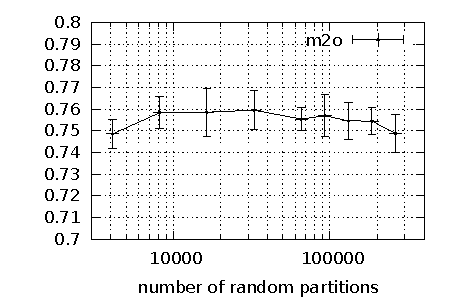
\includegraphics[width=\linewidth]{plot-p.pdf}
\caption{Number of random partitions vs. m2o.}
\label{plot-p}
\end{figure}

Figure~\ref{plot-p} gives results where the number of initial random
partitions is varied over a large range and shows the results to be
fairly stable across two orders of magnitude.

\begin{figure}[ht] \centering
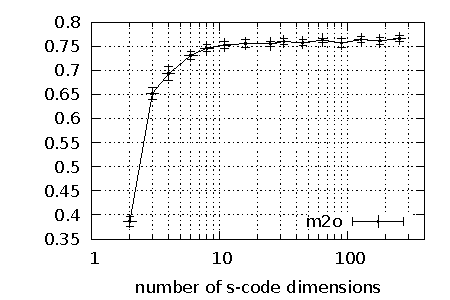
\includegraphics[width=\linewidth]{plot-d.pdf}
\caption{Number of s-code dimensions vs. m2o.}
\label{plot-d}
\end{figure}

Figure~\ref{plot-d} shows that at least 10 embedding dimensions are
necessary to get within 1\% of the best result, but there is no
significant gain from using more than 25 dimensions.

\begin{figure}[ht] \centering
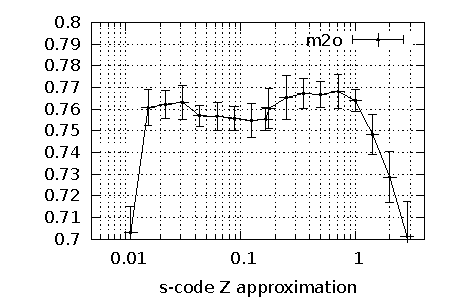
\includegraphics[width=\linewidth]{plot-z.pdf}
\caption{S-code Z approximation vs. m2o.}
\label{plot-z}
\end{figure}

Figure~\ref{plot-z} shows that the constant $\tilde{Z}$ approximation
can be varied within two orders of magnitude without a significant
performance drop in the many-to-one score.  For uniformly distributed
points on a 25 dimensional sphere, the expected $Z\approx 0.146$.  In
the experiments where we tested we found the real $Z$ always to be in
the 0.140-0.170 range.  When the constant $\tilde{Z}$ estimate is too
small the attraction in Eq.~\ref{eq:attract} dominates the repulsion
in Eq.~\ref{eq:repulse} and all points tend to converge to the same
location.  When $\tilde{Z}$ is too high, it prevents meaningful
clusters from coalescing.
%%% I have seen the first, but the second is pure guess, need to
%%% look.  The distances seem to be decreasing on that end as well!

We find the random partition algorithm to be fairly robust to different
parameter settings and the resulting many-to-one score significantly
better than the bigram baseline.

\subsection{Random substitutes}\label{sec:wordsub}

Another way to use substitute vectors in a discrete setting is simply
to sample individual substitute words from them.  The
random-substitutes algorithm cycles through the test data and pairs
each word with a random substitute picked from the pre-computed
substitute vectors (see Section~\ref{sec:lm}).  We ran the
random-substitutes algorithm to generate 50 million word ($X$) --
random-substitute ($Y$) pairs as input to S-CODE.  Clustering the
resulting $\phi_x$ vectors yields a many-to-one score of .7662
(.0066).

This result is close to the previous result by the random-partition
algorithm (.7594) demonstrating that two very different discrete
representations of context based on paradigmatic features give
consistent results.  Both results are significantly above the bigram
baseline.  Figure~\ref{plot-s} illustrates that the random-substitute
result is fairly robust after a couple of million word-substitute
samples.

\begin{figure}[ht] \centering
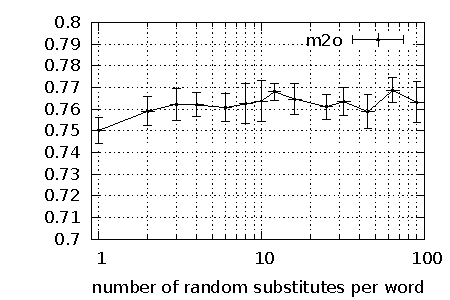
\includegraphics[width=\linewidth]{plot-s.pdf}
\caption{Number of word-substitute samples vs. m2o.}
\label{plot-s}
\end{figure}

\subsection{Adding features}\label{sec:feat}

\subsection{Comparison}\label{sec:comparison}

\section{Error Analsis}

\section{Contributions}
\label{sec:contrib}

We introduced a paradigmatic representation for word context which
contains possible substitutes for the target word and their
probabilities.  The substitute probabilities were estimated using a
standard 4-gram language model with Kneser-Ney smoothing.  We
investigated distance metrics, dimensionality reduction techniques and
clustering algorithms appropriate for substitute probability vectors
and evaluated them using a supervised k-nearest-neighbor baseline and
many-to-one accuracy relative to a 45-tag 24K word test corpus.  We
found that the KL2 distance metric (a symmetric version of
Kullback-Leibler divergence), dimensionality reduction using Laplacian
eigenmaps, and spectral clustering work well with substitute vectors.
Spectral clustering of substitute vectors reveal a grouping that
largely match traditional part of speech boundaries (\spectralResult\%
many-to-one accuracy) which further improve when the one-tag-per-word
constraint is imposed (\collapseResult\% many-to-one accuracy).  These
results compare favorably to previous results published for the 45-tag
24K word test corpus we have used.  
%% We are investigating ways to speed up the algorithm so it can be tested on larger corpora.

\bibliographystyle{acl2012}
\bibliography{posind2012}

\end{document}
